% --------------------------------------------------------------------------------

\begin{exercise}[Exercise 3.19]

The value of an action, $q_\pi(s, a)$, depends on the expected next reward and the expected sum of the remaining rewards.
Again we can think of this in terms of a small backup diagram, this one rooted at an action (state-action pair) and branching to the possible next states:

\begin{center}
    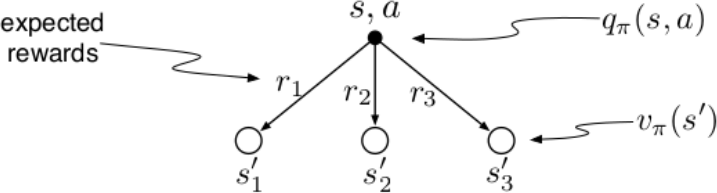
\includegraphics[width = 0.5 \textwidth]{1.19.png}
\end{center}

Give the equation corresponding to this intuition and diagram for the action value, $q_\pi(s, a)$, in terms of the expected next reward, $R_{t+1}$ , and the expected next state value, $v_\pi(S_{t+1})$, given that $S_t = s$ and $A_t = a$.
This equation should include an expectation but not one conditioned on following the policy.
Then give a second equation, writing out the expected value explicitly in terms of $p(s_0, r \mid s, a)$ defined by \eqref{eq:3.2}, such that no expected value notation appears in the equation.

\end{exercise}

% --------------------------------------------------------------------------------

\begin{solution}

\begin{align*}
    q_\pi(s, a)
    & =
    \E_\pi[G_t \mid S_t = s, A_t = a] \\
    & =
    \E_\pi[R_{t+1} + \gamma G_{t+1} \mid S_t = s, A_t = a] \\
    & =
    \sum_{s^\prime, r}
        p(s^\prime, r \mid s, a)
        \E_\pi[R_{t+1} + \gamma G_{t+1} \mid S_t = s, A_t = a, S_{t+1} = s^\prime, R_{t+1} = r] \\
    & =
    \sum_{s^\prime, r}
        p(s^\prime, r \mid s, a)
        E_\pi[r + \gamma G_{t+1} \mid S_t = s, A_t = a, S_{t+1} = s^\prime] \\
    & =
    \sum_{s^\prime, r}
        p(s^\prime, r \mid s, a)
        \pbraces
        {
            r + \gamma \E_\pi[G_{t+1} \mid S_t = s, A_t = a, S_{t+1} = s^\prime]
        } \\
    & =
    \sum_{s^\prime, r}
        p(s^\prime, r \mid s, a)
        (r + \gamma v_\pi(s^\prime)) \\
    & =
    \sum_{s^\prime}
        \pbraces
        {
            p(s^\prime \mid s, a)
            \sum_r
                r
                \frac
                {
                    p(s^\prime, r \mid s, a)
                }{
                    p(s^\prime \mid s, a)
                }
            +
            \gamma v_\pi(s^\prime)
            \sum_r
                p(s^\prime, r \mid s, a)
        } \\
    & =
    \sum_{s^\prime}
        \pbraces
        {
            p(s^\prime \mid s, a)
            r(s, a, s^\prime)
            +
            \gamma v_\pi(s^\prime)
            p(s^\prime \mid s, a)
        } \\
    & =
    \sum_{s^\prime}
        p(s^\prime \mid s, a)
        \pbraces
        {
            r(s, a, s^\prime)
            +
            \gamma v_\pi(s^\prime)
        } \\
    & =
    \E[R_{t+1} + \gamma v_\pi(S_{t+1}) \mid S_t = s, A_t = a]
\end{align*}

\end{solution}

% --------------------------------------------------------------------------------
